\chapter{Evaluation}
\label{chap:evaluation}

\section{Ziel der Evaluation}
Ziel der Evaluation ist es zu überprüfen, ob die in Kapitel \ref{chap:requirements} definierten Anforderungen erfüllt worden sind. Dafür werden Ergebnisse verschiedener Anfragen aus dem Frontend und Performance Messungen zur Auswertung der Check-API unter Last in unterschiedlichen Umgebnungen ausgewertet und verglichen.

\section{Evaluationsumgebung}
Es gibt drei unterschiedliche Umgebungen die für Teste genutzt wurden. Angefangen mit der lokalen Umgebung auf meinem eigenen Laptop mit 16GB Arbeitsspeicher und dem M1 Pro Chip mit 6 Leistungs- und 2 Effizienzkernen wurde die Check-API einzeln über das Docker-Image lokal ausgeführt. Die zweite Umgebung ist die aktuelle Live-Version, welche zu diesem Zeitpunkt aus dem Deployment mit Docker-Compose besteht und damit alle Services in eigenen Containern laufen. Eine genaue Information über Systemressourcen steht nicht zur Verfügung. Die dritte Umgebung ist eine Kubernetes Umgebung, welche im Rahmen der Bachelorarbeit \texttt{Von Docker Compose zu Kubernetes: Evaluation der Zuverlässigkeit} \cite{baKonstantin} von Konstantin Göke zeitgleich zu dieser entwickelt wurde. Wie auch in der Docker-Compose Umgebung ist bei der Kubernetes Umgebung keine Information über die Hardware bekannt. Die Kubernetes Umgebung nutzt für die Check-API bis zu 4 Pods, welche jeweils bis zu 2000m CPU nutzen können. Für die Leistungsüberprüfung wurde das Tool Gatling \cite{gatling} für Scala genutzt, mit welchem Testfälle und Metriken definiert werden können. Damit die Vergleiche möglichst realistisch und vergleichbar bleiben, wurden zwei Endpunkte in den Systemen genutzt, Es wurde speziell ein Endpunkt in der Haupt-API eingebaut, mit welchem direkt die Check-API, über den gleichen Weg wie auch im normalen Betrieb aufgerufen werden kann. Das wurde notwendig, da die Kubernetes Umgebung die Check-API nicht ohne weiteres nach außen erreichbar macht. Mehr dazu im Abschnitt \ref{sec:evalRobustheit}. Die Teste schicken je nach Endpunkt perfekt abgeschnittene Anfragen an den jeweiligen Endpunkt. Gatling verfügt dabei über die Einstellung, wie viele Nutzer es über einen gewissen Zeitraum geben soll. Ein Nutzer schickt dabei immer alle im Test vorhandenen Anfragen ab, wartet auf eine Antwort und schaltet sich ab. mit der Codezeile \texttt{constantConcurrentUsers(20).during(2.minutes)} werden so z.~B. durch Gatling versucht zwei Minuten lang konstant 20 Nutzer gleichzeitig zu halten. Wird ein Nutzer fertig, startet Gatling direkt einen neuen Nutzer, der erneut den gleichen Prozess durchläuft. Gatling speichert dabei unterschiedliche Werte und erstellt nach Fertigstellung des Test eine Zusammenfassung mit all diesen Werten. Auf diese Werte wird sowohl im Abschnitt \ref{sec:evalRobustheit} und \ref{sec:performance} eingegangen.

\section{Funktionale Evaluation}
\label{sec:functionalEval}
Wie Die Tabelle \ref{tab:functional-evaluation} zeigt, werden die einzelnen Fehlerfälle unterschieden und in dem gewünschten Format ausgegeben. Besonders relevant ist die Ausgabe über verbotene Schlüsselwörter, da dies zeigt, dass bekannte kirtische Befehle erkannt und vor der Ausführung abgefangen werden. Auch die versteckten Tests schlagen an und werden dabei in dem gewünschten generischen Format ausgegeben. Für jeden Fehlerfall wurde im Frontend entsprechender Code geschrieben, abgeschickt und mit dem erwarteten Fehlercode und dem Inhalt der Rückmeldung verglichen.

  \begin{table}[htbp]
	\centering
	\caption{Funktionale Testfälle der Check-API}
	\label{tab:functional-evaluation}
	\begin{tabular}{p{4cm} p{5cm} p{4cm}}
		\textbf{Testfall} & \textbf{Erwartetes Verhalten} & \textbf{Ergebnis} \\
		\hline
		Korrekte Einreichung & Rückgabe von \texttt{200 OK} & Erfolgreich \\
		Kompilierungsfehler & Fehlerklassifikation \texttt{compilation} & Erfolgreich \\
		Fehlgeschlagener öffentlicher Test & Ausgabe einer verständlichen Fehlermeldung & Erfolgreich \\
		Fehlgeschlagener Hidden Test & Generische Fehlermeldung ohne Testdetails & Erfolgreich \\
		Endlosschleife & Abbruch nach Timeout & Erfolgreich \\
		Verbotenes Schlüsselwort & Abbruch vor der Ausführung & Erfolgreich \\
	\end{tabular}
\end{table}


\section{Evaluation der Robustheit und Verfügbarkeit}
\label{sec:evalRobustheit}
Wie schon in dem vorherigen Absatz \ref{sec:functionalEval} aufgezeigt, wird die Robustheit leicht verbessert durch die Filterung von bösartigen Befehlen. Die Analyse der Unterschiedlichen Systeme hat dabei aufgezeigt das in der Docker-Compose Umgebung ein gravirendes Problem besteht. Sollte der Check-API-Container abstürzen, ist das System zwar darauf ausgelegt den Container erneut zu starten, dabei geht allerdings etwas schief, sodass der Container nicht erneut starten kann. Dieses Problem besteht bei der Kubernetes Umgebung allerdings nicht. Fällt hier einer der Check-API-Pods aus, so wird direkt ein neuer Pod gestartet und kann den Ausfall schnellst möglich wieder ausgleichen. Kubernetes bietet desweiteren den Vorteil, auf unterschiedliche Server verteil und repliziert zu werden, was im verlgeich zu der Docker-Compose Umgebung einen Single Point of Failure verhindern kann.

\section{Performance-Evaluation}
\label{sec:performance}
In diesem Abschnitt werden die Ergebnisse der performance Tests aufgeschlüsselt. Dafür wurden die Lokale, Docker-Compose und die Kubernetes Umgebung verglichen. Die Tests bestanden aus einer einfachen Anfrage, welche perfekt auf die Endpunkte in der Haupt-API und der Check-API abestimmt wurden um möglichst einheitliche Testergebnisse zu erziehlen. Dabei wurde die Systeme einmal mit 50 dauerhaften Nutzern über zwei Minuten und ein mal mit 100 dauerhaften Nutzern über zwei Minuten getestet. In den Abbildungen \ref{fig:performance99}, \ref{fig:performance95} und \ref{fig:performance50} wurde die Antwortzeit der optimierten mit der ursprünglichen Version verglichen. Da ich von der Docker-Compose Umgebung vor der Verbesserung keinen Test ausgeführt hatte, bestehen hier leider keine Daten. Die Messungen deuten auf eine Verbesserung hin, Aufgrund der unterschiedlichen Testumgebungen und teilweise unbekannten Hardware sind die Ergebnisse jedoch nur eingeschränlt direkt vergleichbar. In der Kubernetes Umgebung wird eine Verbesserung von 33\% erziehlt. Das entspricht über 15 Sekunden unterschied. Lokal kann das System sogar eine Verbesserung von fast 70\% erreichen, was über 19 Sekunden differenz entspricht. Lokal muss man allerdings beachten, das es keine Übertragunslatenz zu einem Server gibt und die Kubernetes Umgebung die Anfragen nicht direkt in der Check-API sondern in der Haupt-API erhält, da die Check-API ohne weiteres nicht von außerhalb des Systems erreichbar ist. Dadruch muss ebenfalls etwas mehr Rechenzeit für die Verarbeitung und Weiterleitung der Anfrage berechnet werden. Ebenfalls kann man in den Diagrammen erkennen, das die Docker-Umgebung immer etwas schneller Antwortet als die Kubernetes Umgebung. In der Abbilgung \ref{fig:performance50_100User} wird die Antwortzeit der optimierten Version zwischen Docker-Compose und Kubernetes mit 50 und 100 Nutzern verglichen. Hier wird sichbar, das 50 Nutzer und damit weniger Last auf dem System deutlich bessere Ergebnisse in der Antwortzeit liefern als 100. Die Tests sollen offenbaren, wo die Grenzen des Systems liegen und wie eine realistische Nutzung unter extremen Bedingunen, wie einer Klausur, aussieht. 

\begin{figure}[htbp]
	\centering
	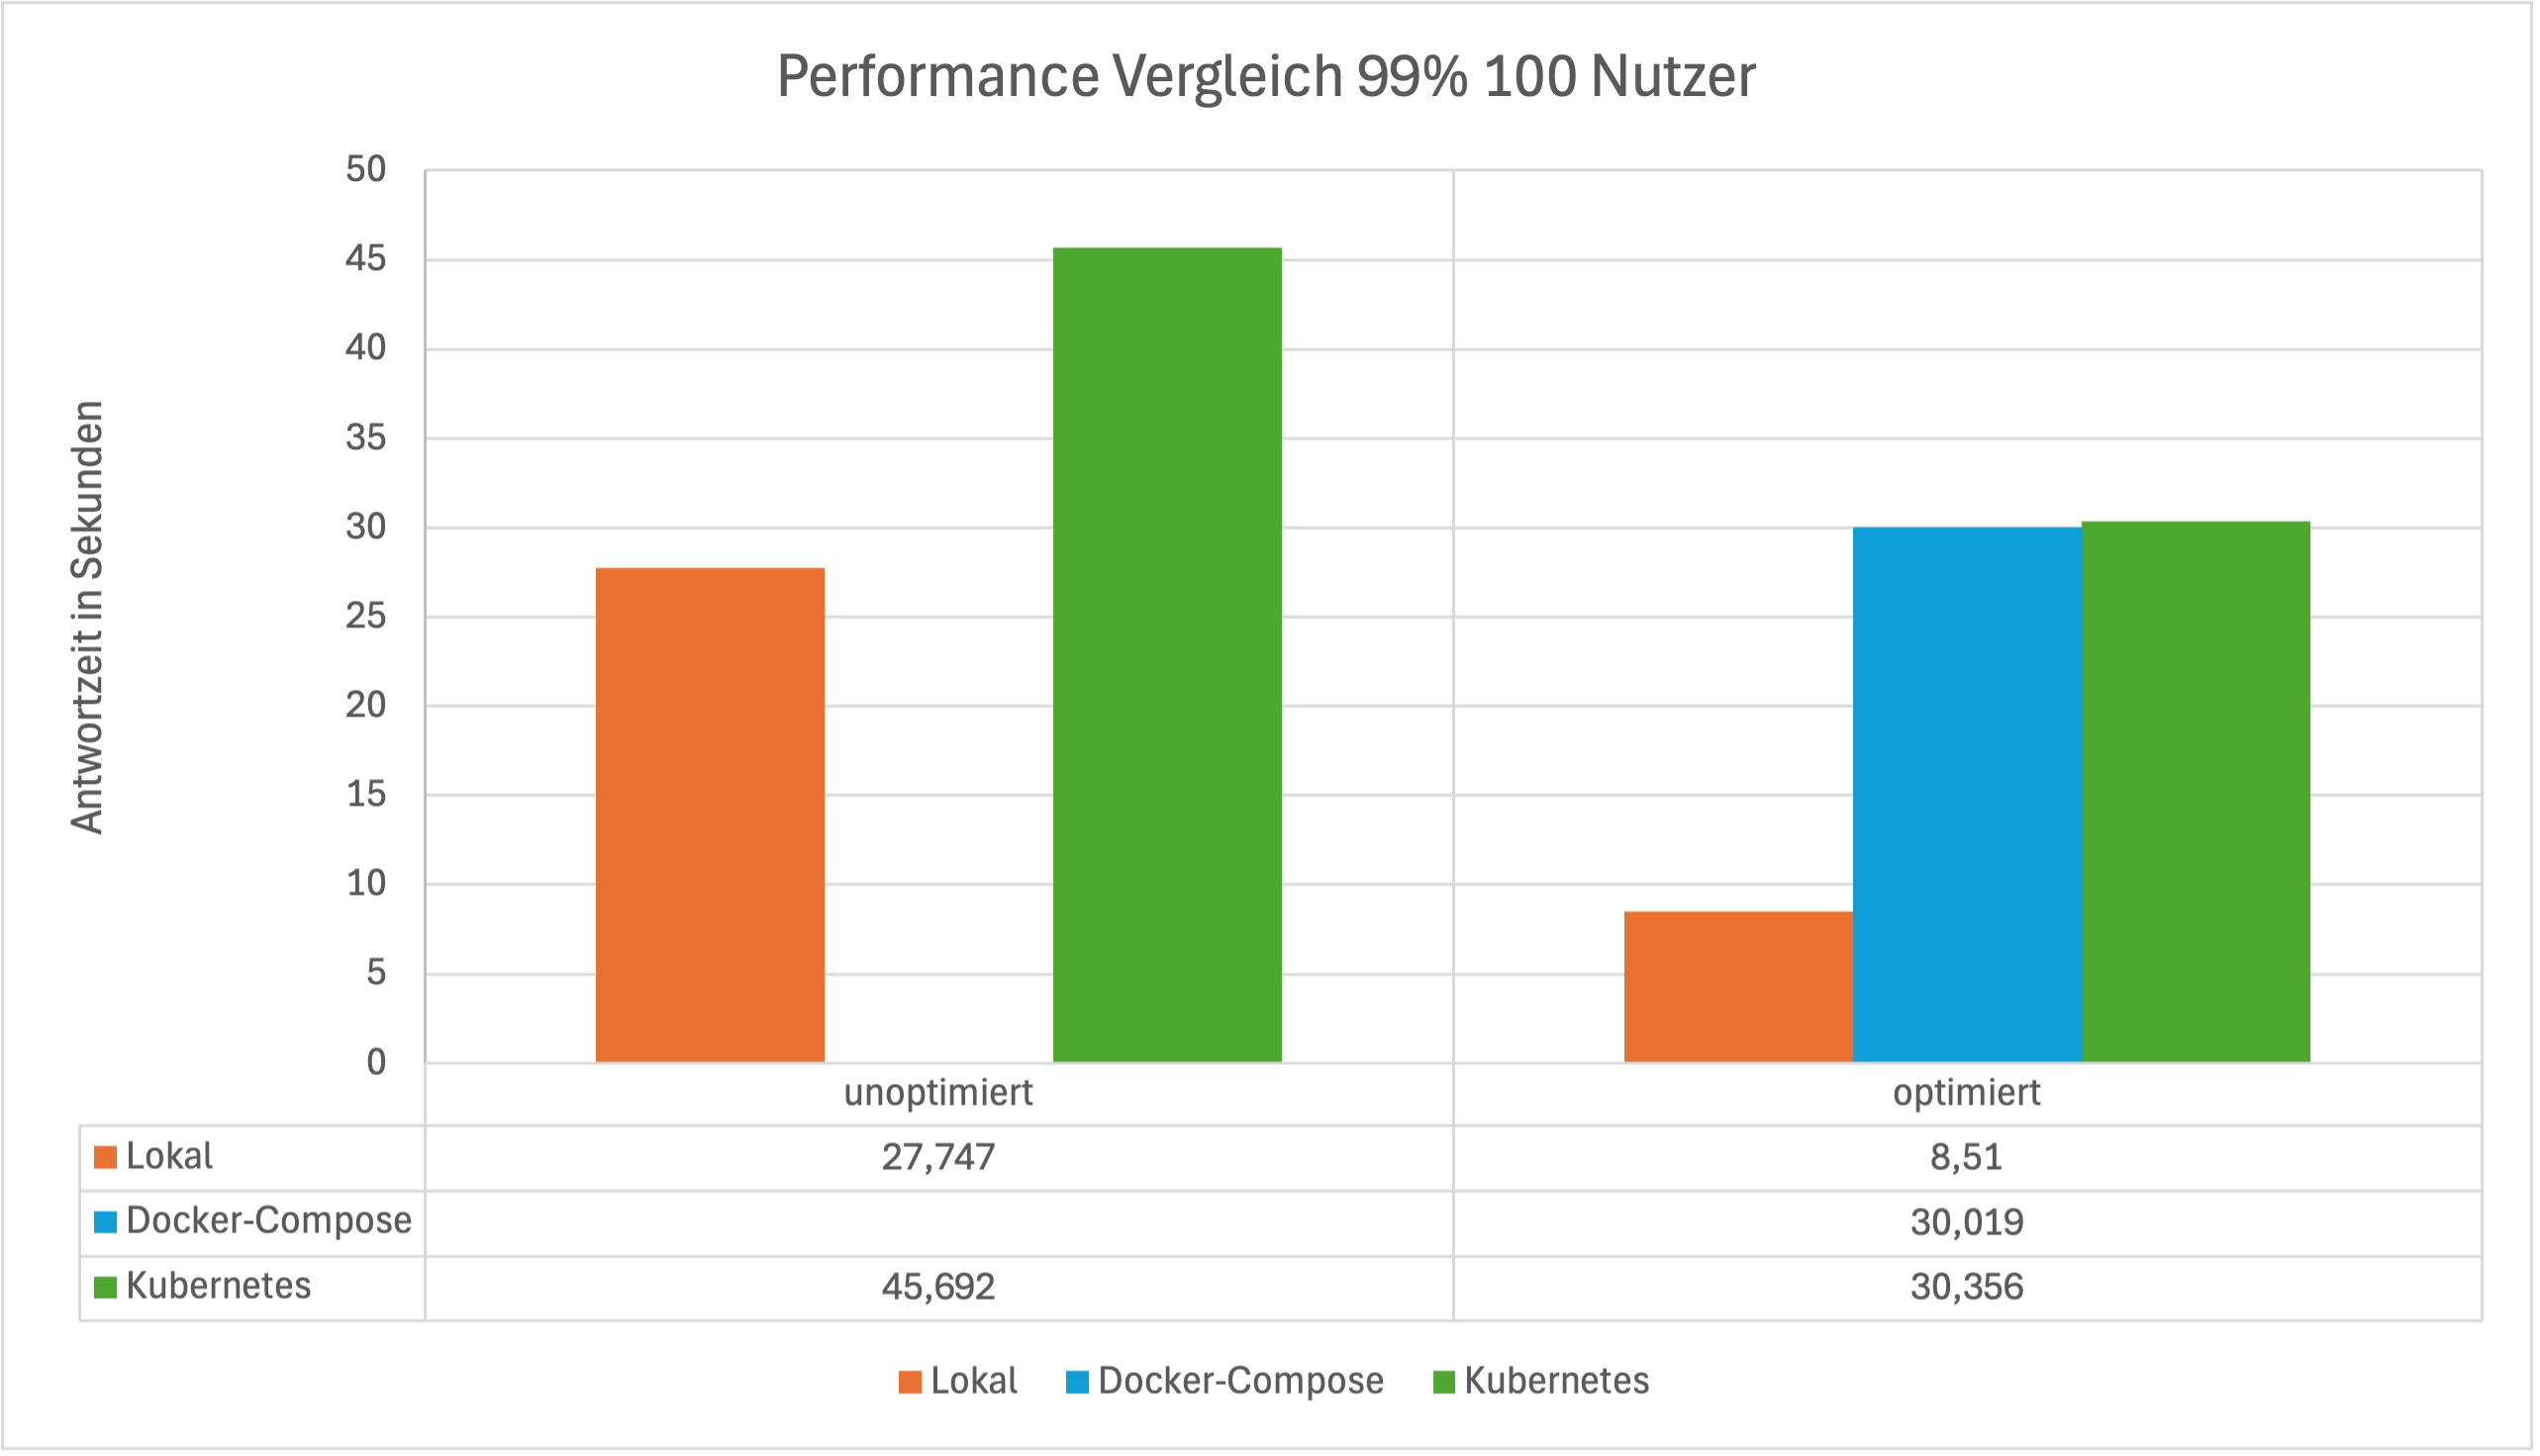
\includegraphics[width=\textwidth]{diagrams/performancevergleich 99 100 Nutzer.png}
	\caption{Performance Vergleich zwischen der Lokalen, Docker-Compose und der Kubernetes Umgebung mit jeweils 100 gleichzeitigen Nutzern im Vergleich die 99. Perzentil der Antwortzeit}
	\label{fig:performance99}
\end{figure}

\begin{figure}[htbp]
	\centering
	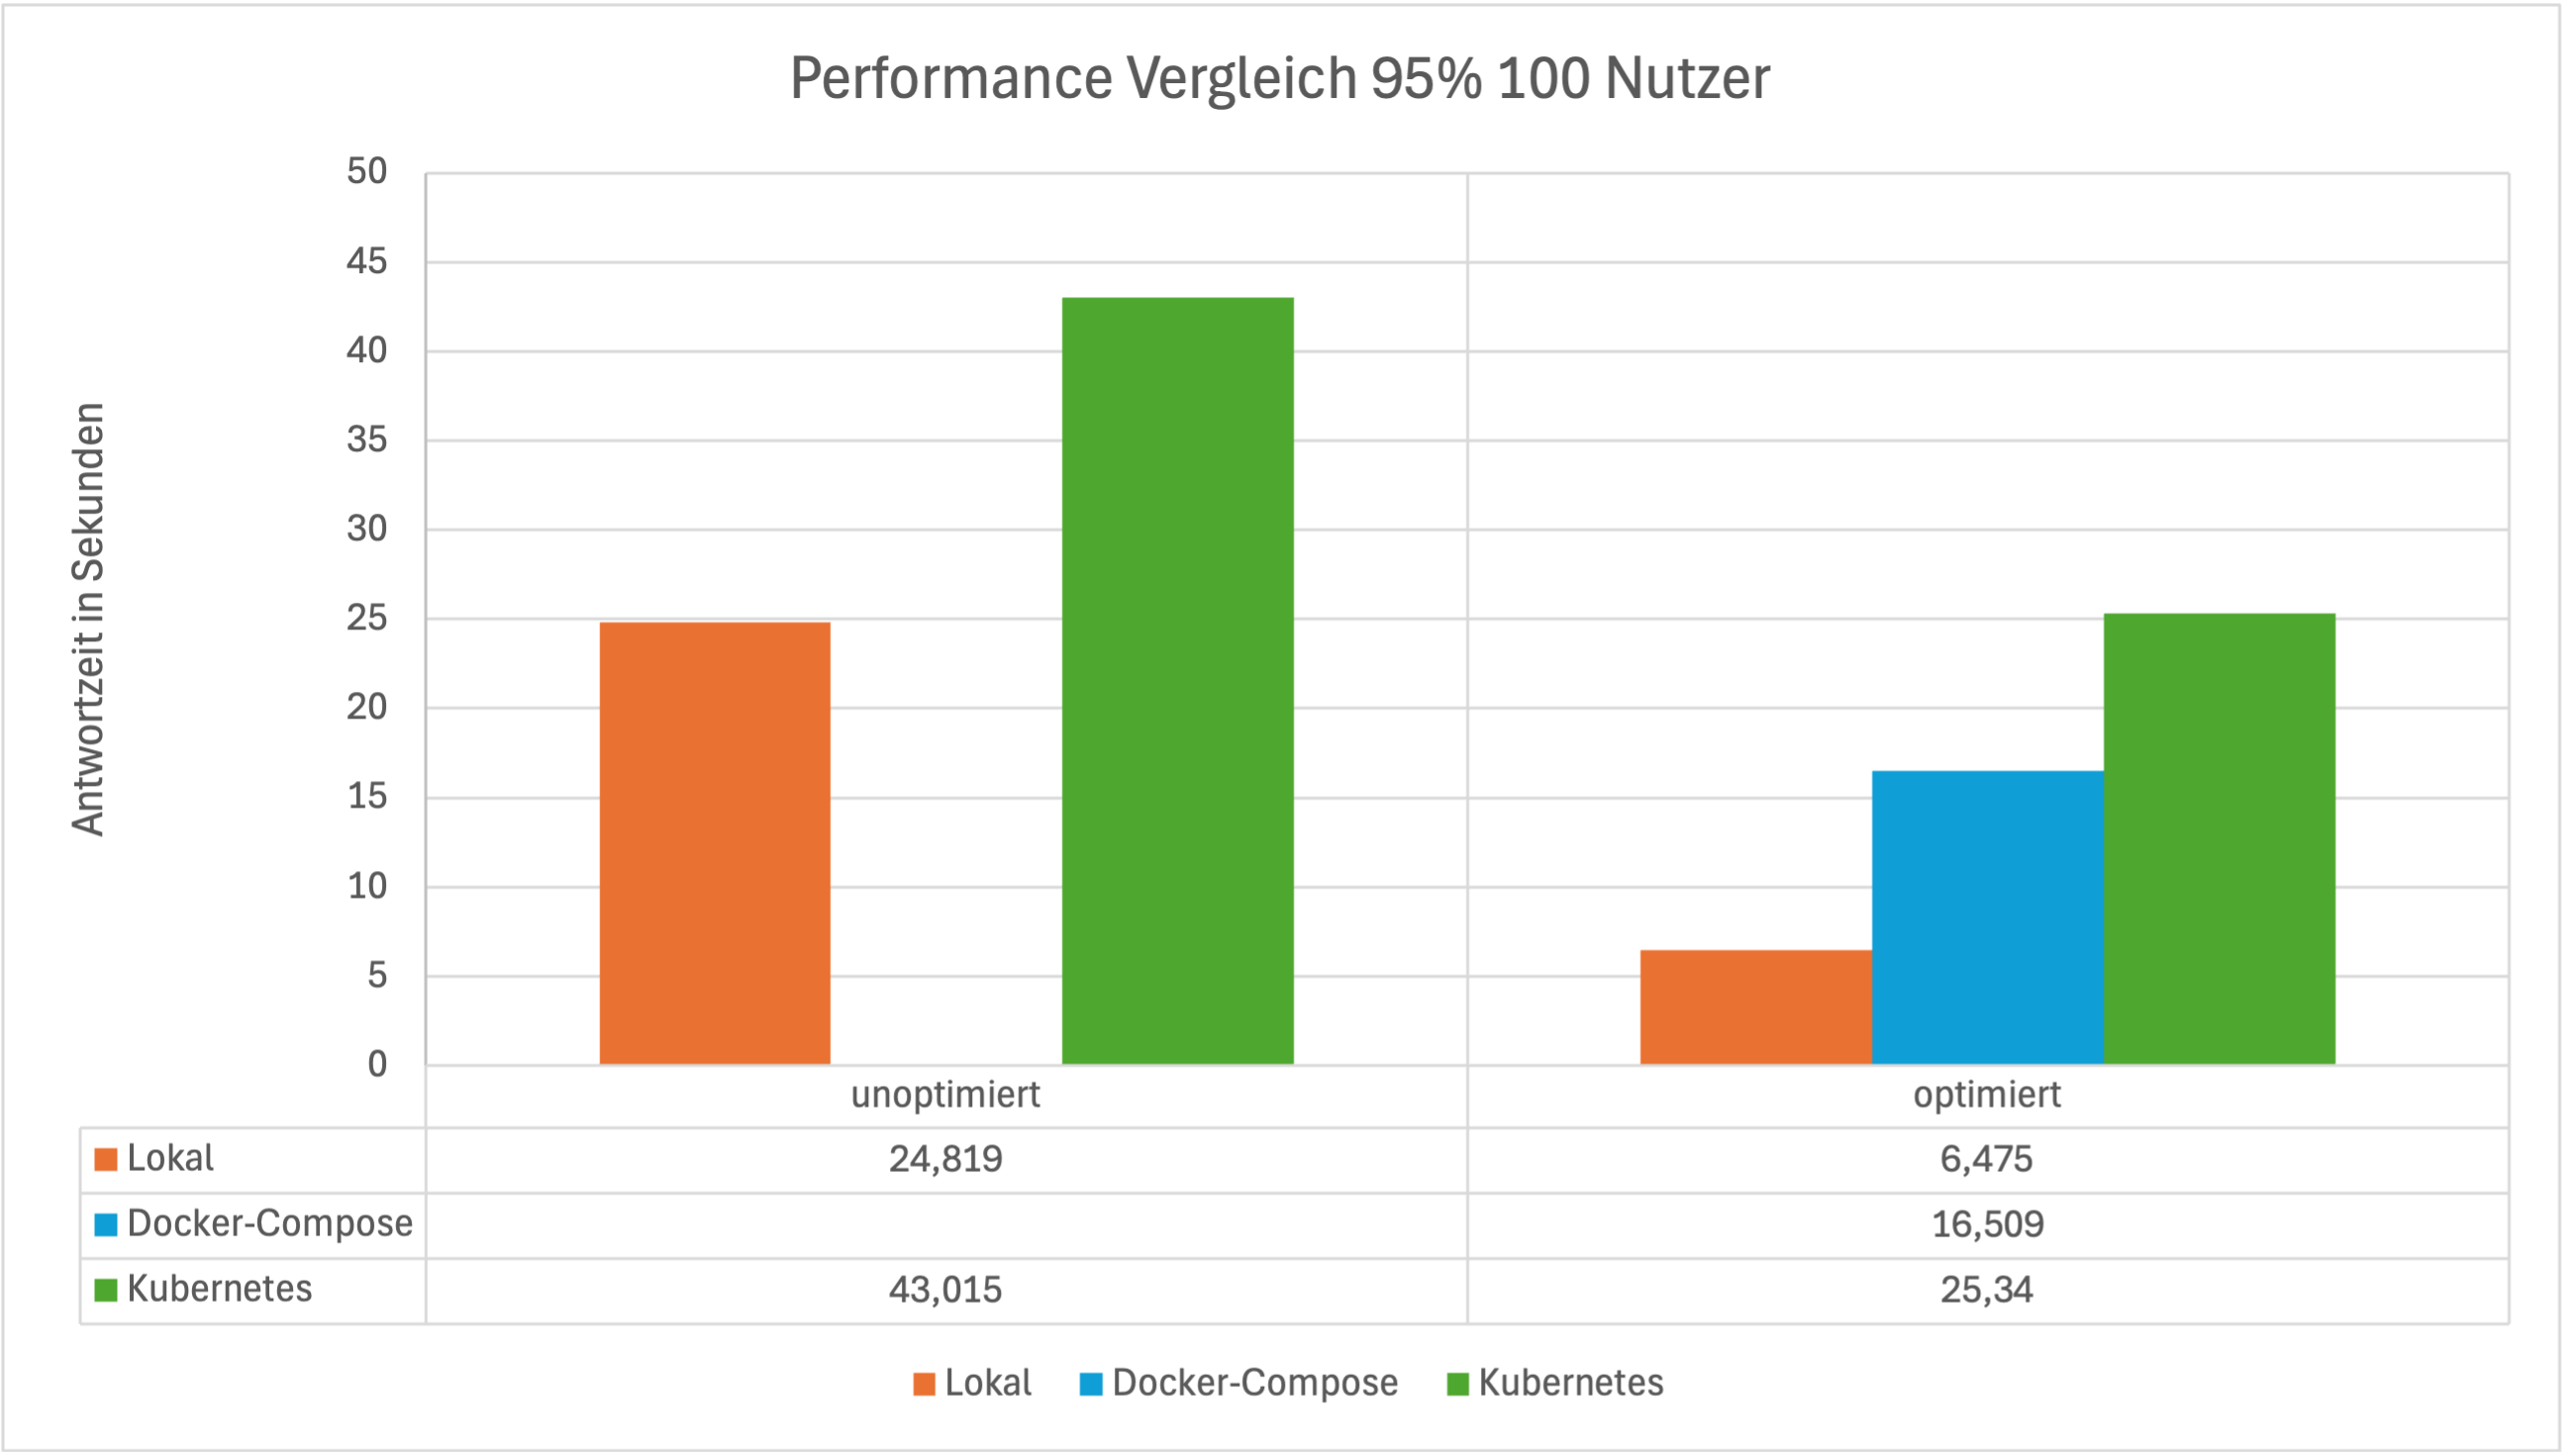
\includegraphics[width=\textwidth]{diagrams/performancevergleich 95 100 Nutzer.png}
	\caption{Performance Vergleich zwischen der Lokalen, Docker-Compose und der Kubernetes Umgebung mit jeweils 100 gleichzeitigen Nutzern im Vergleich die 95. Perzentil der Antwortzeit}
	\label{fig:performance95}
\end{figure}

\begin{figure}[htbp]
	\centering
	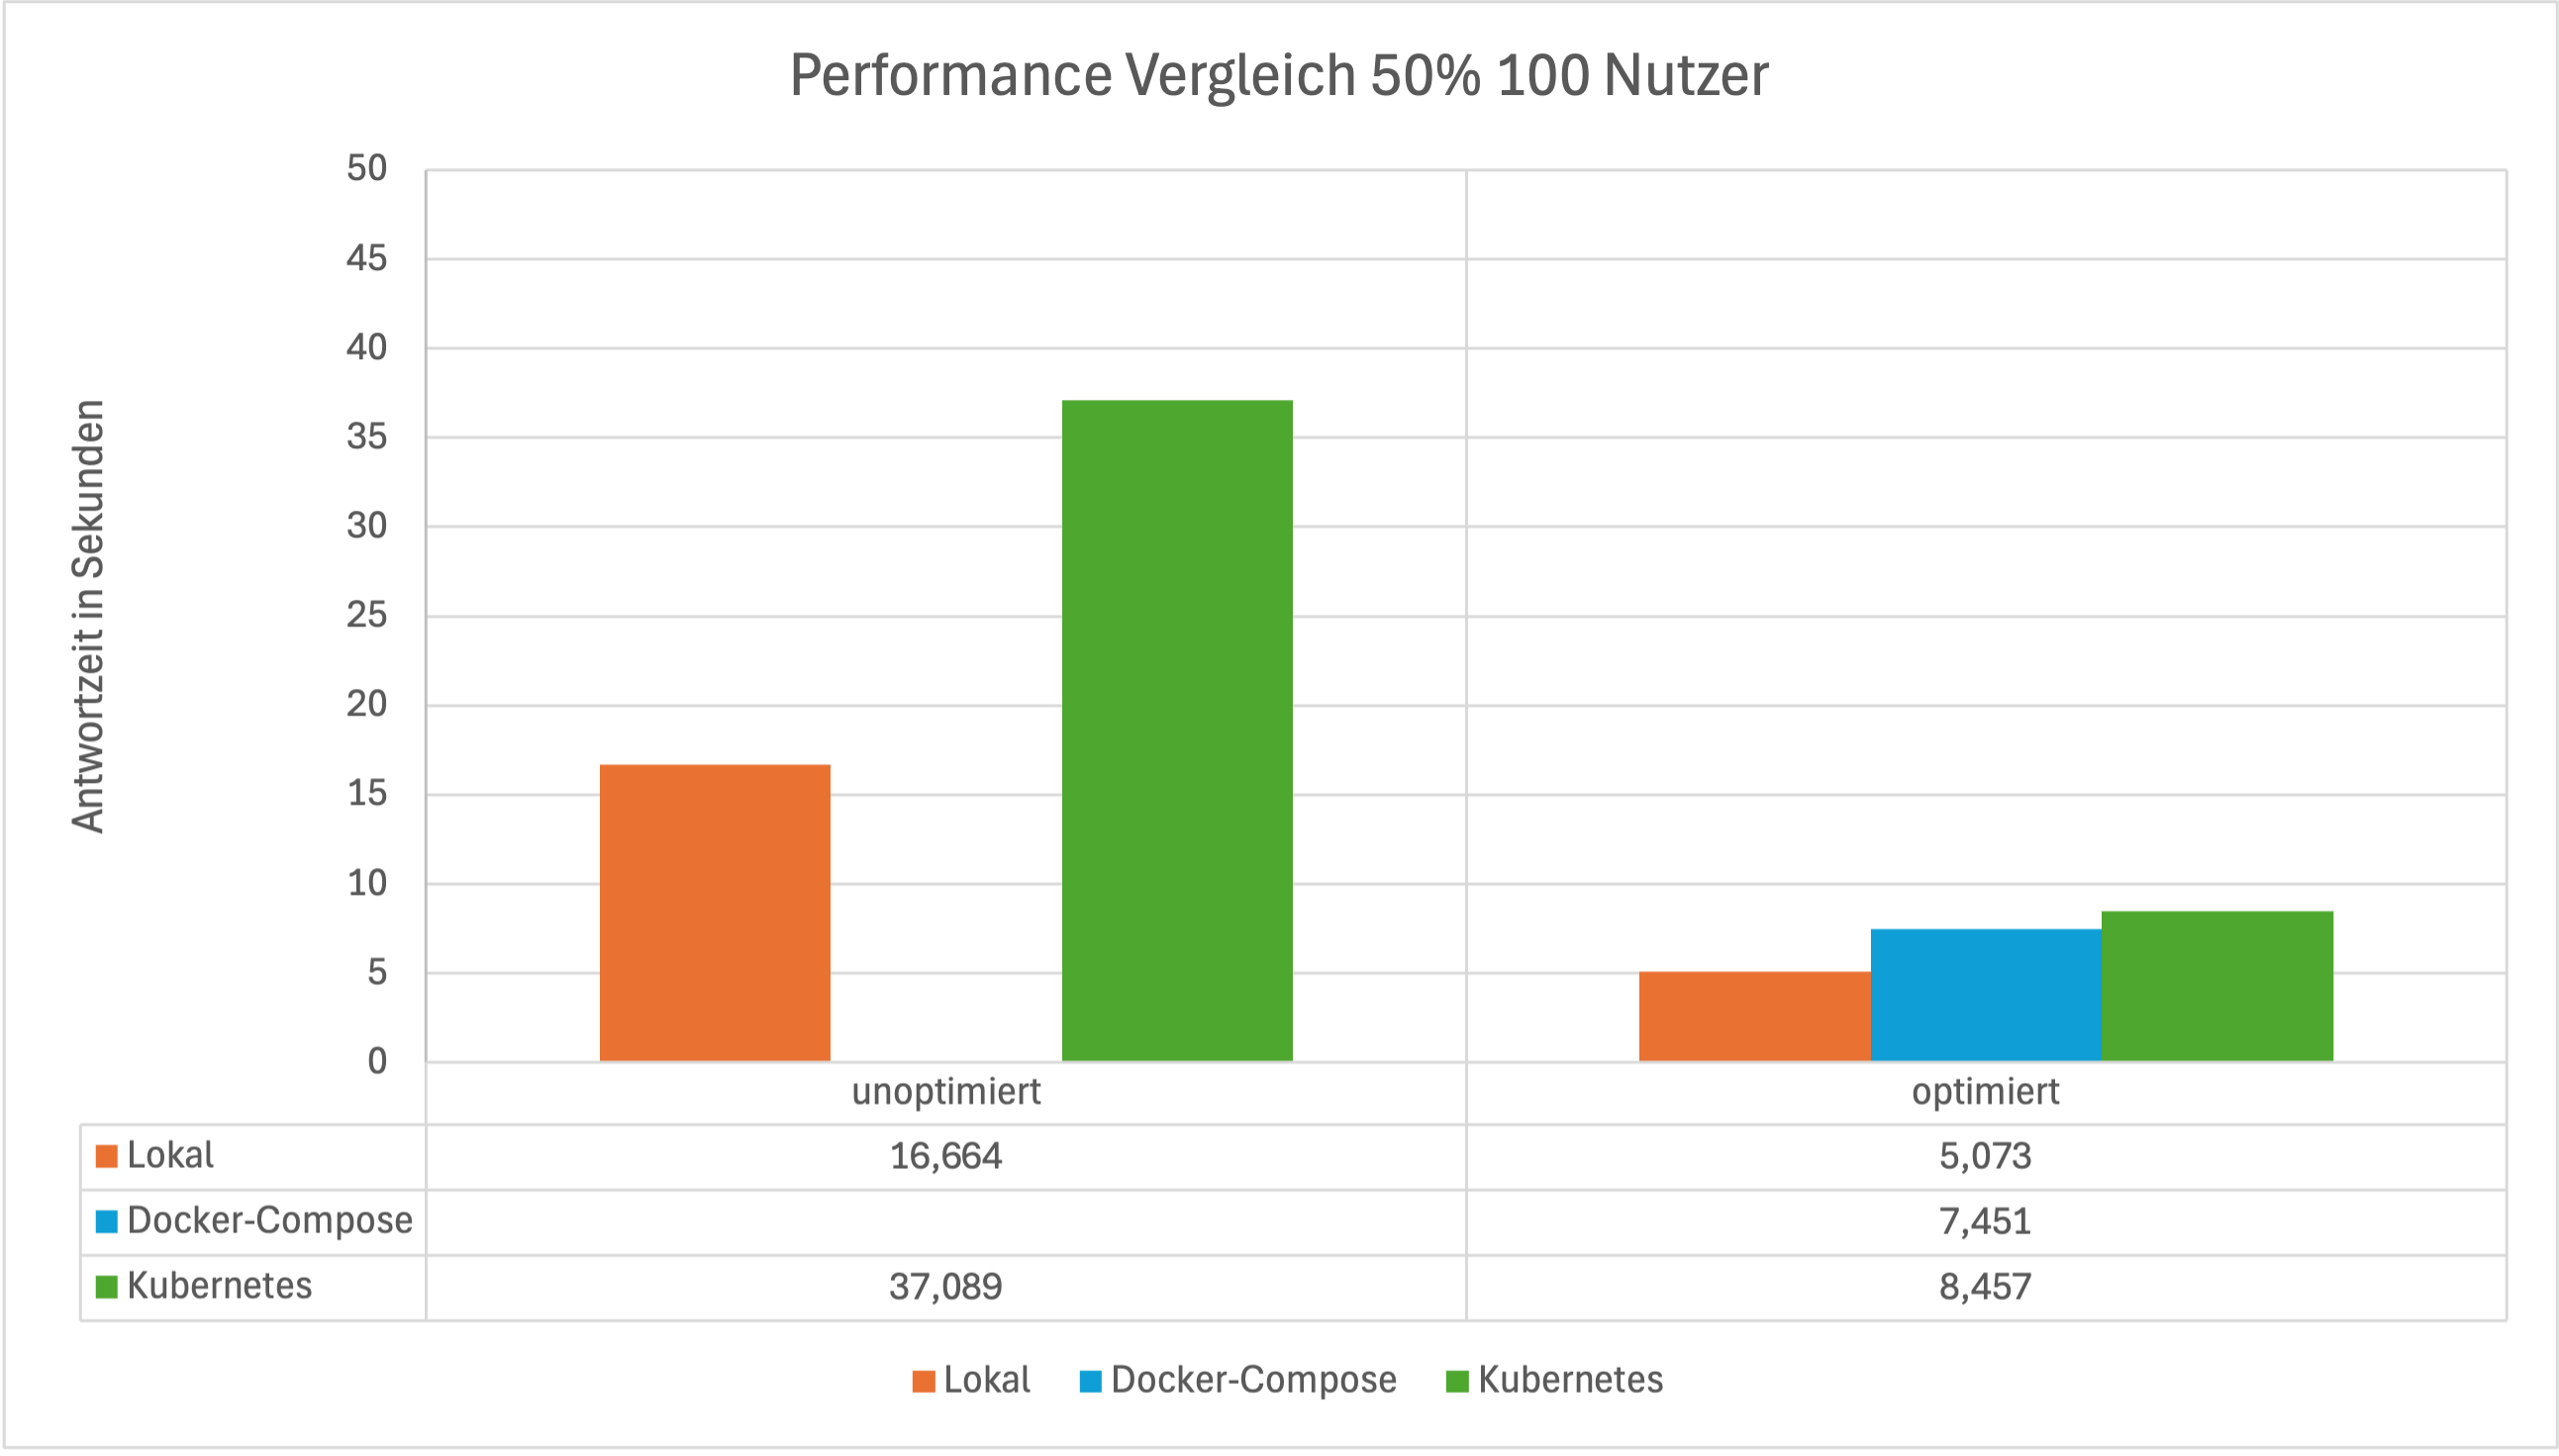
\includegraphics[width=\textwidth]{diagrams/performancevergleich 50 100 Nutzer.png}
	\caption{Performance Vergleich zwischen der Lokalen, Docker-Compose und der Kubernetes Umgebung mit jeweils 100 gleichzeitigen Nutzern im Vergleich die 50. Perzentil der Antwortzeit}
	\label{fig:performance50}
\end{figure}

\begin{figure}[htbp]
	\centering
	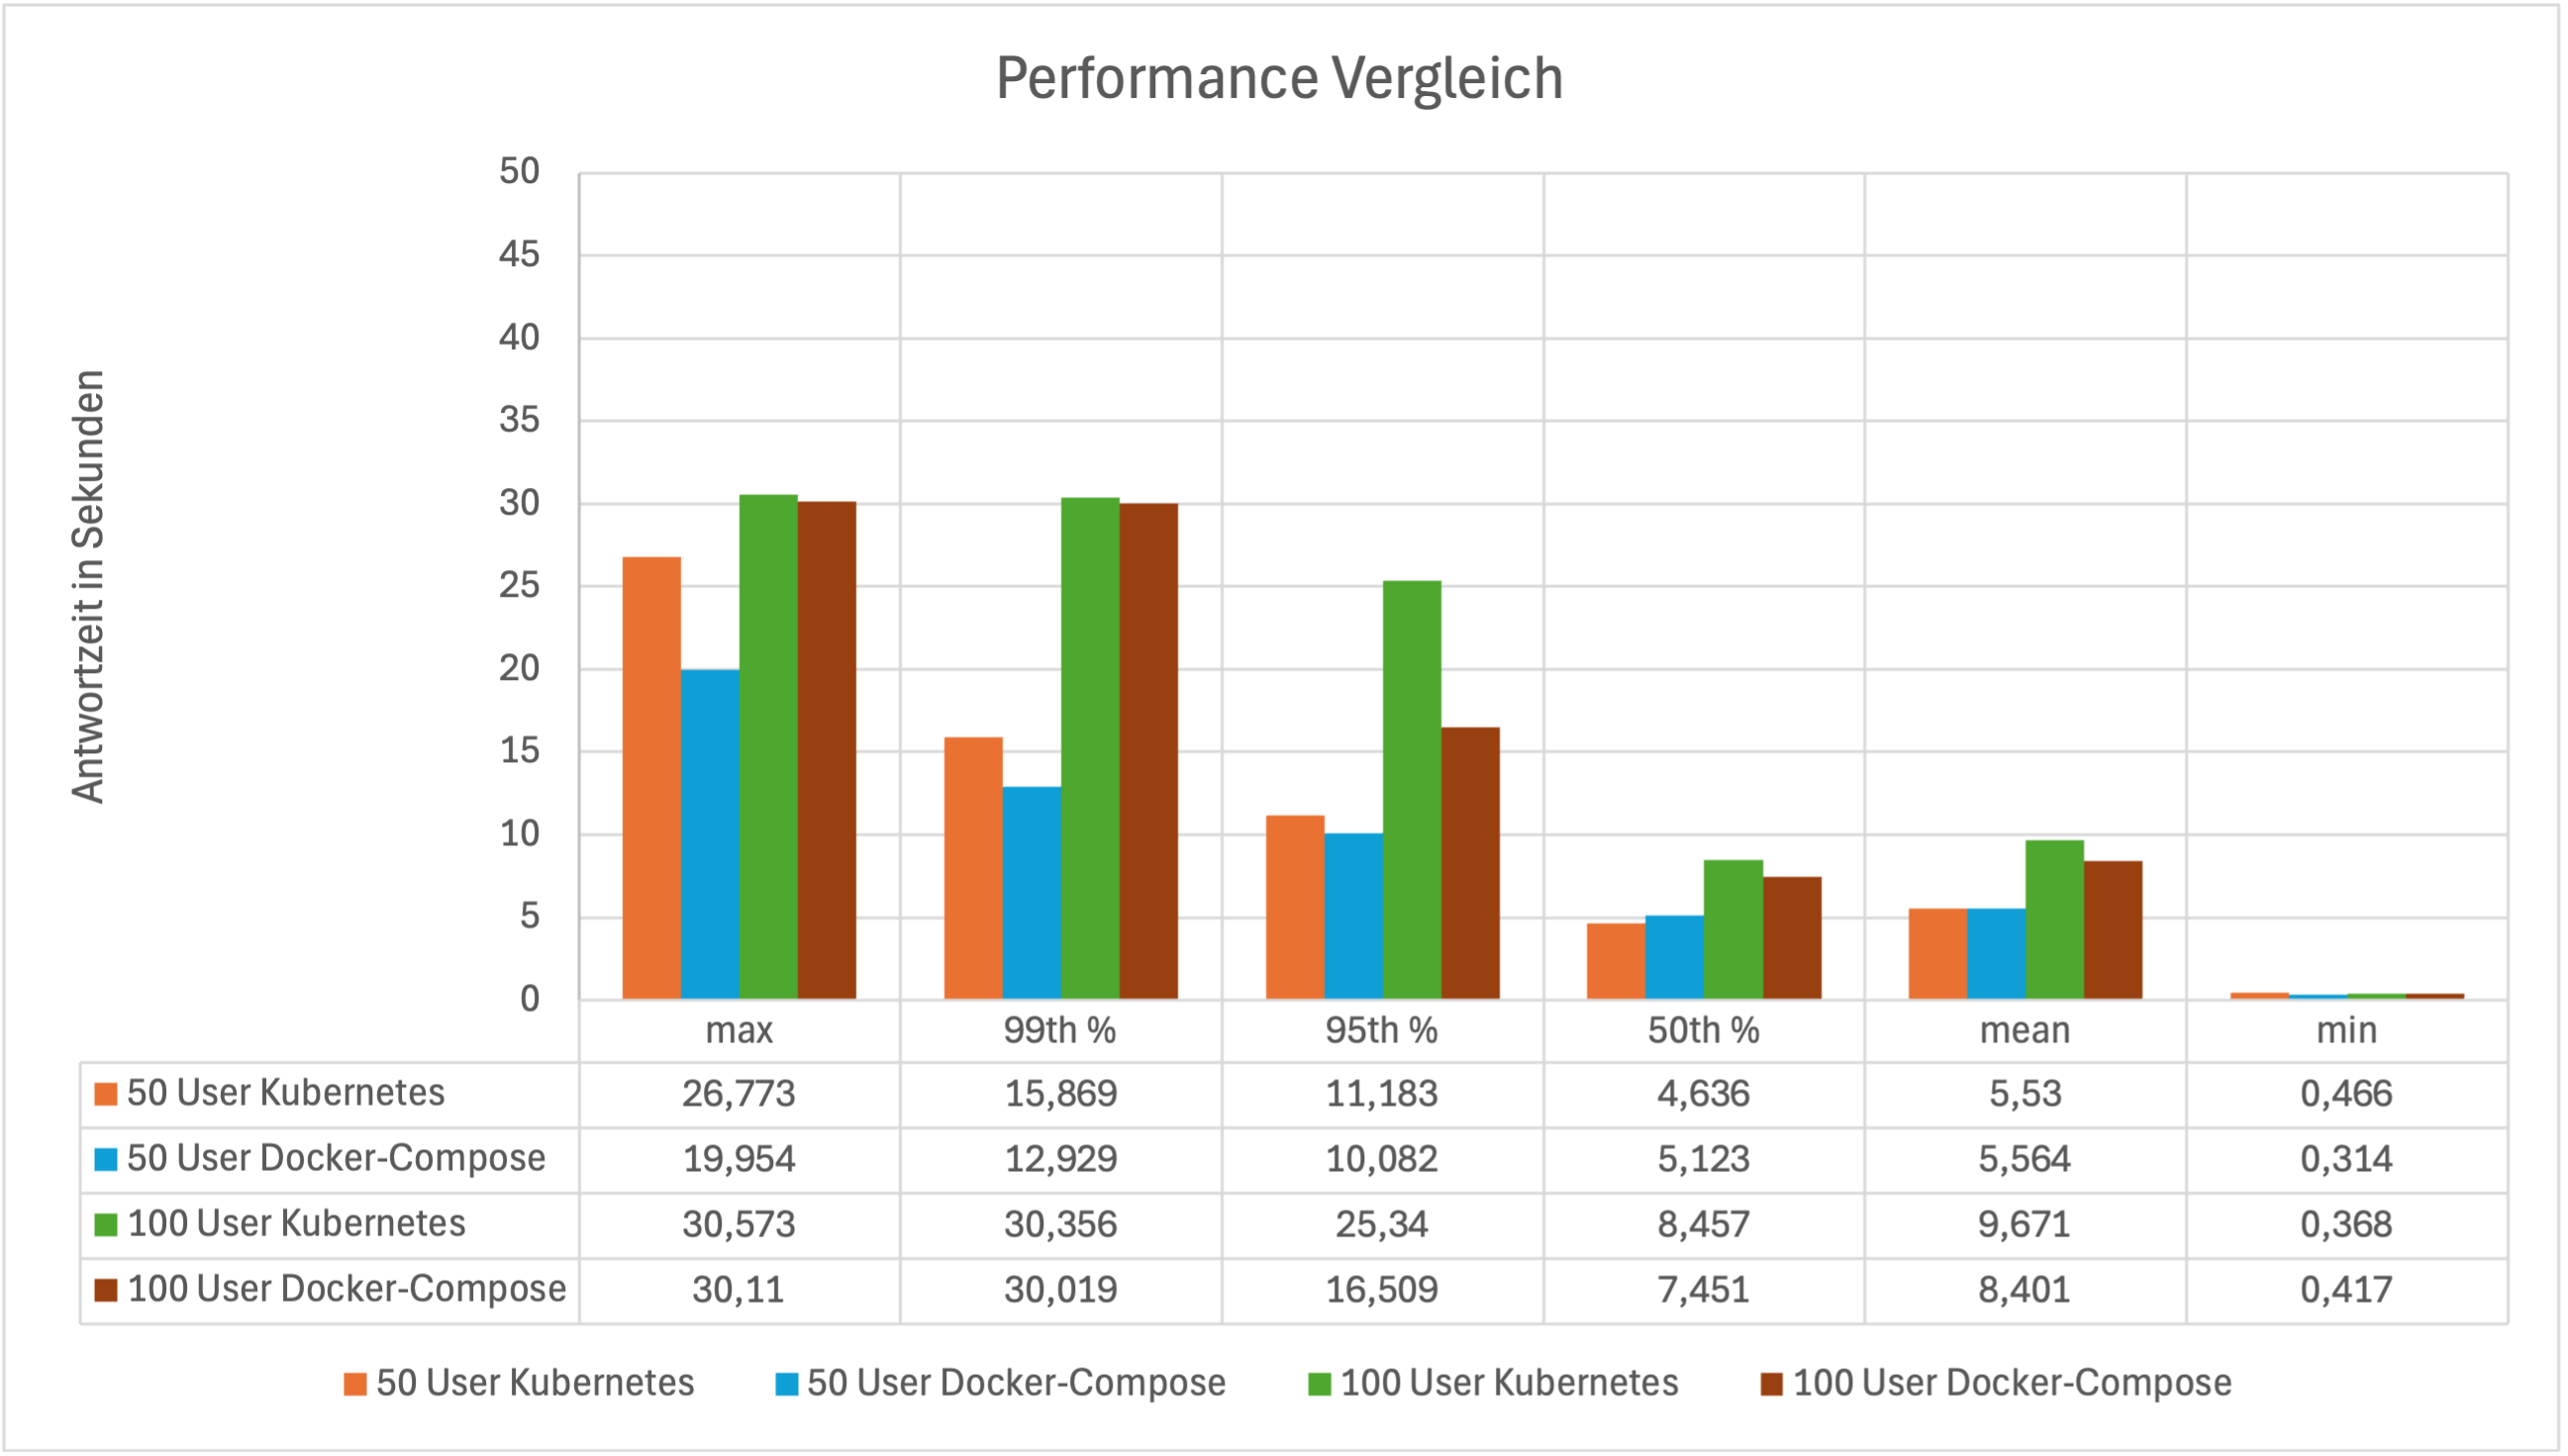
\includegraphics[width=\textwidth]{diagrams/performancevergleich 50 und 100 Nutzer.png}
	\caption{Performance Vergleich zwischen der Docker-Compose und der Kubernetes Umgebung mit jeweils 50 und 100 gleichzeitigen Nutzern}
	\label{fig:performance50_100User}
\end{figure}


\section{Bewertung der Ergebnisse}
Die Ergebnisse zeigen klar, das die Optimierung erfolgreich und notwendig war. Dennoch sind die Ergebnisse unter extrem hoher Auslastung unzureichend. In einer Klausur soll ein Student nicht bis zu über 30 Sekunden auf eine Antwort warten müssen. Obwohl Kubernetes im schlechtesten Fall 53\% schlechter ausfällt aus Docker-Compose, sollte das System dennoch mit Kubernetes weiter entwickelt werden, da mit Kubernetes das System verteilt arbeiten kann und so eine wesentlich bessere Robustheit erhält. Dazu kommt, das mit besserer Hardware oder mehr Ressourcen die Antwortzeiten ebenfalls stark fallen können, wie es der vergleich mit der lokalen Umgebung aufzeigt.
Desweiteren zeigt die Evaluation auf, das versteckte Tests, wie in den Anforderungen, erfolgreich eingebaut wurden und regulär nicht an das Frontend ausgehändigt werden. Die Fehlerfälle werden ebenfalls alle Abgedeckt und sorgen für die gewünschte verbesserte Erläuterung des Fehlers für den Nutzer.

\section{Grenzen der Evaluation}
Die performance Tests wurde mit einem einzigen Testfall durchgeführt und decken keinen vollständigen Betrieb ab. Die gemessenen Werte sind daher abhängig von der Systemkonfiguration, der Hardware und dem genutzen Testfall. Zudem bildet die Evaluation keine vollständige Sicherheitsanalyse gegen alle denkbaren Angriffszenarien ab.
